%!TEX root = ../../secondYearReport.tex
 
\paragraph{Work package 3 progress}

The progress for each task are described hereafter.

\subparagraph{Reproducing existing control results in a simple case (T3.1)}
During year one, UPMC has achieved task T3.1 by creating a stand-alone C++ library encapsulating the whole-body controller developed in \cite{salini2012} so that it can be used by all partners in simulation or on (any) real humanoid robot. This version of the controller has been tested in rigid multi-contact scenarios in simulation (see Fig.~\ref{fig:xde}) and is currently adapted for tests on the iCub robot.


\subparagraph{Formulating the control problem (T3.2)}

The work performed during year one by UPMC to achieve T3.2 has led to the definition of what a task can be considered to be in the context of the reactive formulation of a multi-task whole body control problem. Among the different characteristics of a task (physical frame, task variable, forward model, desired target trajectory, local controller, priority), the notion of task priority has been largely modified with respect to the classical lexicographic task ordering met in the robotics literature and which is particularly appropriate for cascade resolution approaches such as the one recently proposed in \cite{escande2012}. A partial order has been defined such that task priorities can be described for any pair of task $i$ and $j$. This leads to a richer formulation which includes the original one but is also particularly appropriate for describing task insertion and removal processes as well as priority switching between tasks. Further more, this new prioritization paradigm provides a unique way of defining strict and soft hierarchies between tasks. Associated to this work, the notion  of generalized task projector has been introduced. Each task is associated to a projector which is built based on the tasks priorities. The interest of this projector is that it filters the joint space motion associated to a task so that all priorities are respected, being them soft or strict. Details regarding this work are provided in \cite{liu2013}.

Within this task also IIT contributed with the definition of a software abstraction layer, named wholeBodyInterface (\url{http://wiki.icub.org/codyco/dox/html/namespacewbi.html}). This software library defines the interface to access and control the robot  whole-body. Therefore the wholeBodyLibrary structures the control problem and their definition. Currently the library has been been implemented for both the iCub and the Gazebo iCub simulator.  

\subparagraph{Solving the local control problem (T3.3)}

Associated to the new task formulation proposed in T3.2, the control problem has been formulated by UPMC as an LQP which can be solved by any convex optimization solver dealing with linear constraints. Despite the task hierarchy, the introduction of a generalized task projector per task allows to solve only one LQP. This can be done by introducing as many virtual joint space variables as the number of tasks and using the generalized projector of each task in the expression of the constraints. The resulting problem can be solved by standard convex optimization tools and the cost of introducing virtual joint space variables is compensated for by the fact that only one optimization problem has to be solved. Details regarding this work are provided in \cite{liu2013}.

In the meantime, TUD has proposed to explore optimization methods for solving local control problems that do not require the explicit inversion of any model of the system.  During year one, TUD investigated Bayesian optimization methods that were applied to bipedal locomotion tasks.  One of the key challenges in robotic bipedal locomotion is finding gait parameters that optimize a desired performance criterion, such as speed, robustness or energy efficiency. Typically, gait optimization requires extensive robot experiments and specific expert knowledge. During year one, TUD demonstrated that  data-driven machine learning methods based on Bayesian optimization can be used to automate and speed up the process of gait optimization. These Bayesian optimization methods were used to efficiently find gait parameters that optimize the desired performance metric on a real bipedal walker \cite{calandra2014} and \cite{calandra2014b}.
    

\subparagraph{Bootstrapping and validating the control approach in rigid world and compliant cases (T3.4)}

During year one, UPMC has explored the contribution of MPC approaches to handle the postural balancing problem under varying contact conditions. The hybrid nature of the problem, where varying contact conditions can be accommodated either by adapting the internal forces distribution given a set of contact or by modifying the set of contacts itself, requires control approaches where the desired task trajectories performed through the local, reactive, whole-body controller have to be optimally planned ahead of time in order to provide robust behaviors. The contributions in this domain are mostly related to the work of A. Ibanez \cite{ibanez2013}, \cite{ibanez2014-icra} and \cite{ibanez2014-ark}. The originality of theses contributions lies in:
\begin{itemize}
	\item an augmented ZMP model including external forces exerted directly on indirectly on the center of mass;
	\item a distributed optimization approach that provides a way of generating reference trajectories for the center of mass representing a good compromise given some antagonistic balance and task;
	\item a non scripted foot step placement optimization.
\end{itemize}

UPMC also partially contributed with an experimental study about human behavior during physical contact with the robot. The protocol was registered and obtained the approval of the ethics committee CERES (Conseil d’\'evaluation \'ethique pour les recherches en sant\'e), from University Paris-Decartes. \footnote{Ivaldi et al., "Engagement during human-humanoid interaction", IRB N. 20135200001072.}
The purpose of the experiments is to collect a database of behaviors of experts and naive people interacting physically with the iCub to accomplish a cooperative task. The collected data also include locations of contacts (retrieved through the tactile skin), applied force, robot mouvements: they will be used to study adaptation to human intention during human-robot physical contacts.
    
In the meantime, TUD investigated the interchange of forces during cooperative tasks between humans and robots \cite{berger2013}. Three example scenarios are illustrated in Figure \ref{fig:interaction_tasks}. In such tasks, typically an exchange of forces takes place whenever the interacting agents make contact. Sometimes, forces are even exchanged through an object that is manipulated by both agents, e.g., through a box that is lifted. For a successful execution of such joint physical activities, a robot needs to accommodate for the external forces exerted by a human. To this end, we developed a machine learning approach for identifying external influences and guidance information from humans. During behavior execution by a robot, predictions from a statistical sensor model are continuously compared with stability parameters derived from current sensor readings. Differences between predicted and measured values exceeding the variance of the statistical model are interpreted as perturbations caused by a human and are used to adapt the robot's behavior.

%!TEX root = ../../thirdYearReport.tex

Continuing the activities which started in the first year of the project, IIT further improved the torque whole-body controller. During the third year of the project, attention was mainly on rigid contacts even if the theoretical and software development was guided and constrained by the requirements for extending the approach to non-rigid contacts. Several improvements to the controller significantly improved its performances. Improvements include in-situ force/torque sensor calibration \cite{Traversaro2015b}, inertial parameter identification \cite{Traversaro2015} and individual motor transfer function identification \cite{Nori2015a}. These improvements made possible quite challenging control tasks like the robust single foot balancing represented in Fig.~\ref{fig:footBalancing}. Details of the controller will be given in a forthcoming publication\footnotetext{\url{https://www.youtube.com/watch?v=SYVCbzGsBF4}.}. 

\begin{figure}[h]
\vspace{0.5em}
\centering
{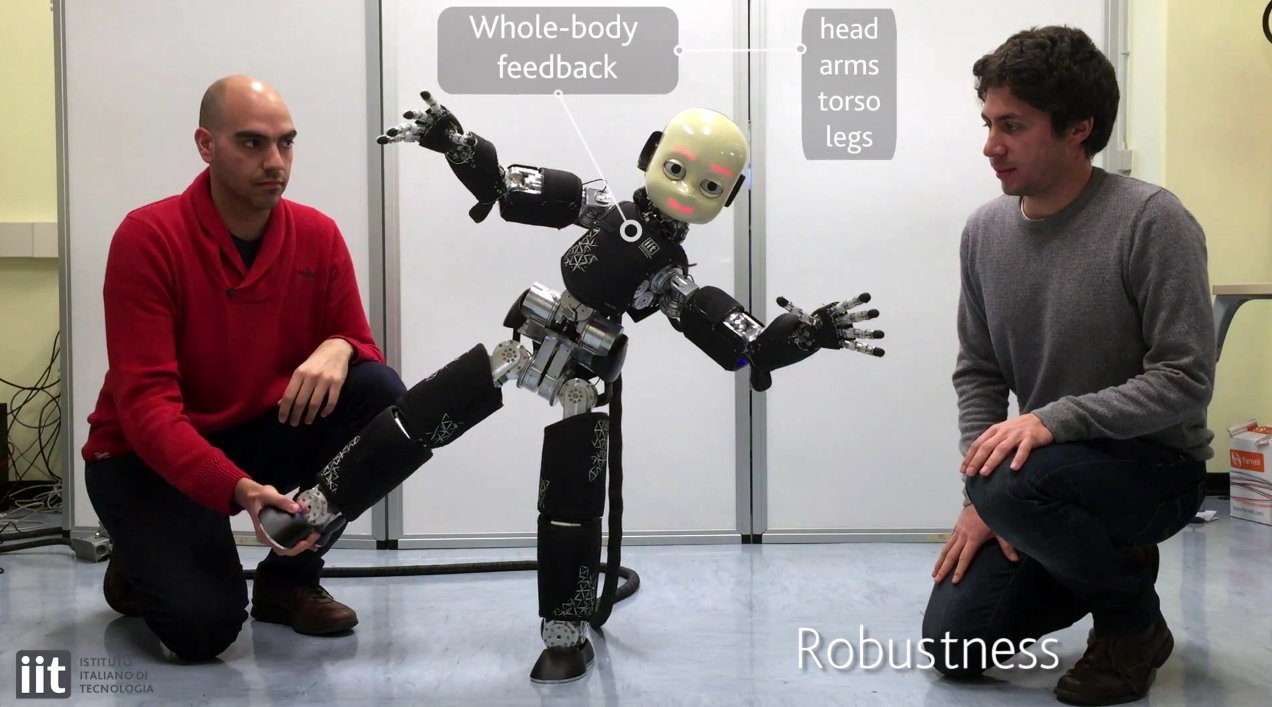
\includegraphics[width=0.65\textwidth]{images/single_foot_balancing.jpg}}
\caption{The picture shows the iCub while performing compliant single foot balancing. Details on the controller can be found in \cite{Nori2015a}. A video of the task is available on youtube\protect\footnotemark.}
\label{fig:footBalancing}
\end{figure}



    
\subparagraph{Deviations from workplan}  

The PM expenses for WP3 after one year of project are globally conform to the planned one. The observed deviations are related to the fact that tasks 3.3 and 3.4 spans the overall duration of the project and the contribution of some of the partners are expected in the 2nd, 3rd and 4th year.

%\emph{\color{red}[For work package 3 (UPMC) provide the following information:]}
%\begin{itemize}
%\item[-] \emph{\color{red}[A summary of progress towards objectives and details for each task;]}
%\item[-] \emph{\color{red}[Highlight clearly significant results;]}
%\item[-] \emph{\color{red}[If applicable, explain the reasons for deviations from Annex I and their impact on other tasks as well as on available resources and planning;]}
%\item[-] \emph{\color{red}[If applicable, explain the reasons for failing to achieve critical objectives and/or not being on schedule and explain the impact on other tasks as well as on available resources and planning (the explanations should be consistent with the declaration by the project coordinator) ;]}
%\item[-] \emph{\color{red}[a statement on the use of resources, in particular highlighting and explaining deviations between actual and planned  person-months per work package and per beneficiary in Annex 1 (Description of Work);]}
%\item[-] \emph{\color{red}[If applicable, propose corrective actions.]}
%\end{itemize}




